% SonicVitals -- signal-processing pipeline (vector figure).
% Build:  pdflatex fig_pipeline.tex
% Dashed amber blocks = target design, not yet implemented. Set
% \markplannedfalse once the code matches the paper.
\documentclass[tikz,border=4pt]{standalone}
\usepackage{amsmath}
\usepackage{newtxtext,newtxmath}
\usetikzlibrary{arrows.meta,positioning,calc,shapes.geometric}

\newif\ifmarkplanned
\markplannedfalse

\definecolor{navy}{RGB}{0,40,85}
\definecolor{blue}{RGB}{0,98,155}
\definecolor{lightblue}{RGB}{232,241,250}
\definecolor{amber}{RGB}{200,110,20}
\definecolor{red}{RGB}{180,40,40}
\definecolor{green}{RGB}{0,128,80}

\ifmarkplanned
  \tikzset{planned/.style={dashed, draw=amber}}
\else
  \tikzset{planned/.style={}}
\fi

\begin{document}
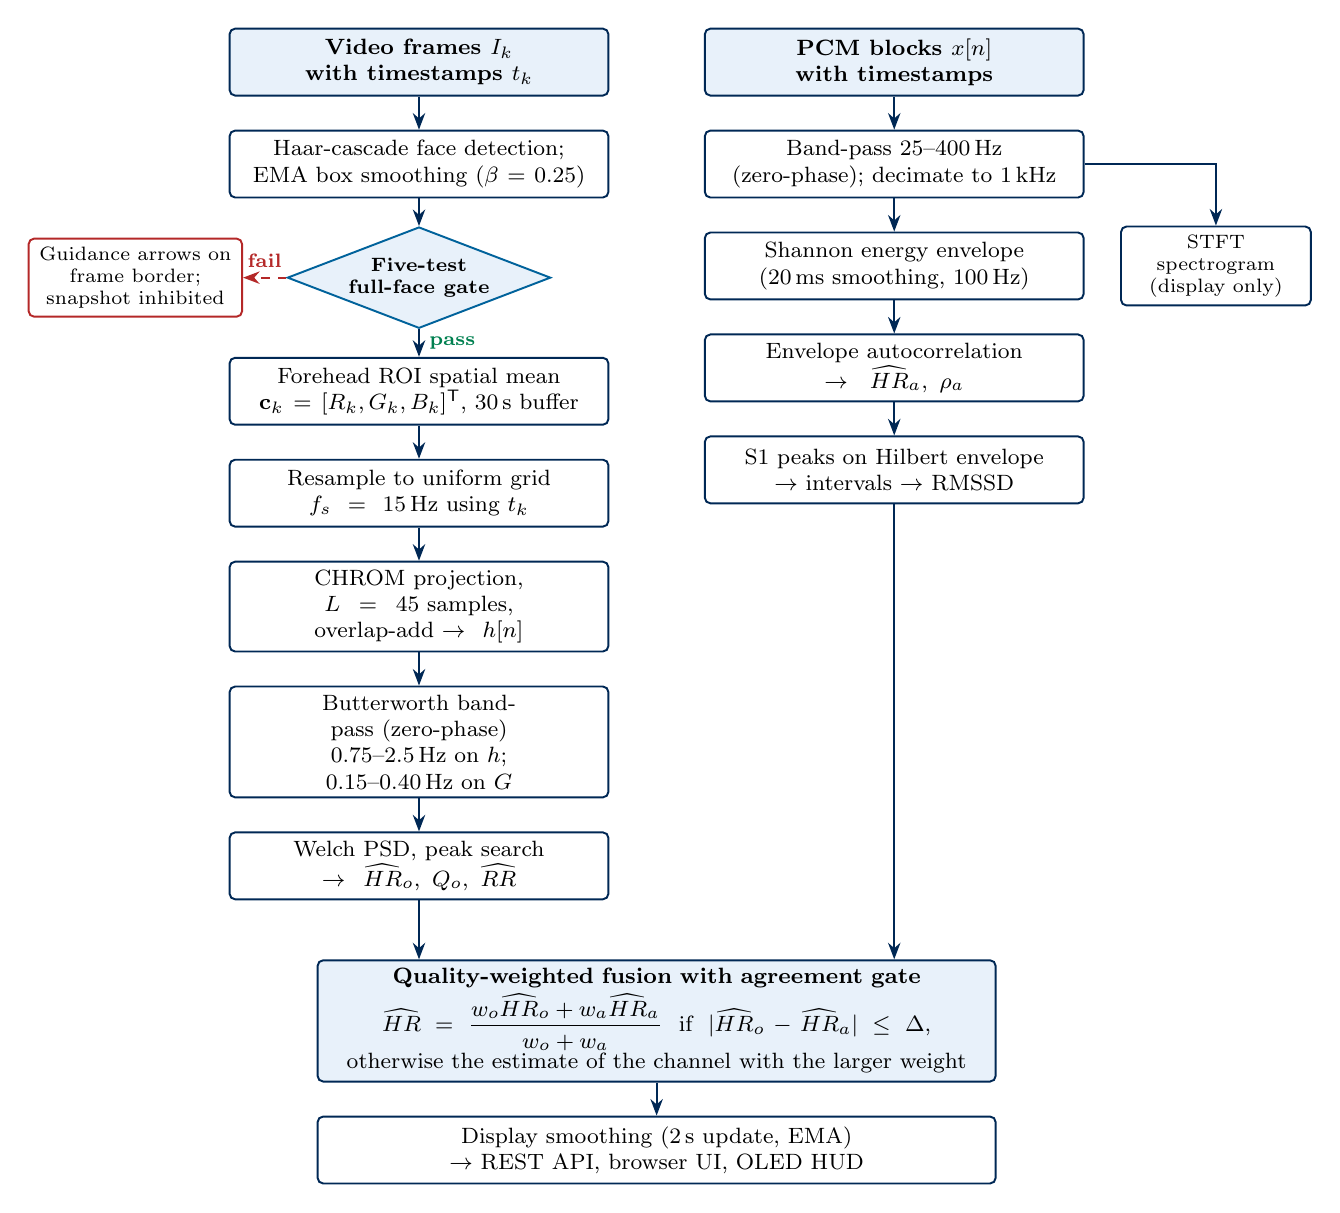
\begin{tikzpicture}[
  font=\footnotesize,
  >={Stealth[length=2.1mm]},
  node distance=0.42cm,
  stp/.style={draw=navy, fill=white, rounded corners=2pt, line width=0.7pt,
              align=center, text width=4.6cm, inner sep=3pt, minimum height=0.85cm},
  src/.style={stp, fill=lightblue, font=\footnotesize\bfseries},
  dec/.style={draw=blue, fill=lightblue, diamond, aspect=2.6, align=center,
              inner sep=1pt, font=\scriptsize\bfseries, line width=0.7pt},
  side/.style={draw=red, fill=white, rounded corners=2pt, align=center,
               text width=2.5cm, inner sep=3pt, font=\scriptsize, line width=0.7pt},
  arr/.style={->, line width=0.75pt, draw=navy}
]
% ------------------------------------------------------------ optical column
\node[src] (o0) {Video frames $I_k$ with timestamps $t_k$};
\node[stp, below=of o0] (o1) {Haar-cascade face detection;\\ EMA box smoothing ($\beta = 0.25$)};
\node[dec, below=0.35cm of o1] (o2) {Five-test\\ full-face gate};
\node[stp, below=0.35cm of o2] (o3) {Forehead ROI spatial mean\\ $\mathbf{c}_k = [R_k, G_k, B_k]^{\mathsf T}$, 30\,s buffer};
\node[stp, below=of o3, planned] (o4) {Resample to uniform grid\\ $f_s = 15$\,Hz using $t_k$};
\node[stp, below=of o4] (o5) {CHROM projection, $L = 45$ samples,\\ overlap-add $\rightarrow h[n]$};
\node[stp, below=of o5] (o6) {Butterworth band-pass (zero-phase)\\ 0.75--2.5\,Hz on $h$;\; 0.15--0.40\,Hz on $G$};
\node[stp, below=of o6] (o7) {Welch PSD, peak search\\ $\rightarrow \widehat{HR}_{o},\ Q_{o},\ \widehat{RR}$};

\node[side, left=0.55cm of o2] (g) {Guidance arrows on\\ frame border;\\ snapshot inhibited};

% ------------------------------------------------------------ acoustic column
\node[src, right=1.2cm of o0] (a0) {PCM blocks $x[n]$ with timestamps};
\node[stp, below=of a0, planned] (a1) {Band-pass 25--400\,Hz\\ (zero-phase); decimate to 1\,kHz};
\node[stp, below=of a1, planned] (a2) {Shannon energy envelope\\ (20\,ms smoothing, 100\,Hz)};
\node[stp, below=of a2, planned] (a3) {Envelope autocorrelation\\ $\rightarrow \widehat{HR}_{a},\ \rho_{a}$};
\node[stp, below=of a3, planned] (a4) {S1 peaks on Hilbert envelope\\ $\rightarrow$ intervals $\rightarrow$ RMSSD};
\node[side, draw=navy, right=0.45cm of a2, text width=2.2cm] (a5) {STFT\\ spectrogram\\ (display only)};

% ------------------------------------------------------------ merge
\coordinate (mid) at ($(o7.south)!0.5!(a4.south |- o7.south)$);
\node[stp, planned, text width=8.4cm, below=0.75cm of mid, fill=lightblue, font=\footnotesize]
  (f) {\textbf{Quality-weighted fusion with agreement gate}\\[1pt]
       $\widehat{HR}=\dfrac{w_o\widehat{HR}_o+w_a\widehat{HR}_a}{w_o+w_a}$\ \ if\ \ $|\widehat{HR}_o-\widehat{HR}_a|\le\Delta$,\\
       otherwise the estimate of the channel with the larger weight};
\node[stp, text width=8.4cm, below=of f] (out)
  {Display smoothing (2\,s update, EMA) $\rightarrow$ REST API, browser UI, OLED HUD};

% ------------------------------------------------------------ arrows
\draw[arr] (o0) -- (o1);
\draw[arr] (o1) -- (o2);
\draw[arr] (o2) -- node[right, font=\scriptsize\bfseries, text=green] {pass} (o3);
\draw[arr, draw=red, dashed] (o2) -- node[above, font=\scriptsize\bfseries, text=red] {fail} (g);
\draw[arr] (o3) -- (o4);
\draw[arr] (o4) -- (o5);
\draw[arr] (o5) -- (o6);
\draw[arr] (o6) -- (o7);
\draw[arr] (a0) -- (a1);
\draw[arr] (a1) -- (a2);
\draw[arr] (a2) -- (a3);
\draw[arr] (a3) -- (a4);
\draw[arr] (a1.east) -| (a5.north);
\draw[arr] (o7.south) -- (o7.south |- f.north);
\draw[arr] (a4.south) -- (a4.south |- f.north);
\draw[arr] (f) -- (out);

\ifmarkplanned
\node[anchor=north east, font=\scriptsize] at ([yshift=-3pt]out.south east)
  {\tikz[baseline=-0.6ex]{\draw[amber,dashed,line width=0.7pt,rounded corners=1pt] (0,-0.1) rectangle (0.55,0.12);}
   \ planned in target design, not yet implemented};
\fi
\end{tikzpicture}
\end{document}
